\section{PIC Implementation}

Implementing PIC into SINATRA was completed using the algorithm seen in Section \ref{sec:algorithm}. Two important factors were critical during implementation: robustness and efficiency. SINATRA is built to be able to simulate many different fluid scenarios chosen by the user. Therefore, the PIC portion should also have this generality. Therefore, even though the Finite Difference method requires equal cell sizes, the rest of the algorithms are based on the individual cells so that when the mesh is non-uniform the simulation could be updated with minimum work. It was also implemented in an efficient manner for the DSMC setup and algorithms found in SINATRA. This means it used flattened arrays, the built-in particle and cell index arrays, and allowed for easy parallelization. 

\subsection{Finite Difference}
\label{sec:finite_diff}

\indent Finite Difference was chosen as the method to discrete Poisson's equation. Finite difference is a simple and common method for discrediting the Poisson equation and is common in PIC codes. There are other algorithms which could be used, but Finite Difference allows for a relatively simple implementation. The derivation below is for a 7 point finite difference for the Poisson equation \cite{FD_GS} \cite{FDM}.

Starting with the Poisson equation expanded out to each of the 3 directions. 

\begin{equation}
    \label{eqn:poisson_expanded}
    \nabla^2 \phi = \frac{\partial^2 \phi}{\partial x^2} + \frac{\partial^2 \phi}{\partial y^2} + \frac{\partial^2 \phi}{\partial z^2} = - \frac{\rho}{\epsilon_0}
\end{equation}

% Make those 
Next, assuming discretization upon nodes designated by \(i \: \text{,} \: j \: \text{and} \: k\) representing nodes in the \(x \: \text{,} \: y \: \text{and} \: z\) directions respectively \cite{FD_GS}. 

\begin{equation}
    \label{eqn:x_partial}
    \frac{\partial^2 \phi}{\partial x^2}(x_i,y_i,z_i) \approx \frac{1}{h^2}(\phi(x_{i-1},y_j,z_k) - 2\phi(x_i,y_j,z_k) + \phi(x_{i+1},y_j,z_k)),
\end{equation}
\begin{equation}
    \label{eqn:y_partial}
    \frac{\partial^2 \phi}{\partial x^2}(x_i,y_i,z_i) \approx \frac{1}{h^2}(\phi(x_i,y_{j-1},z_k) - 2\phi(x_i,y_j,z_k) + \phi(x_i,y_{j+1},z_k)),
\end{equation}
\begin{equation}
    \label{eqn:z_partial}
    \frac{\partial^2 \phi}{\partial x^2}(x_i,y_i,z_i) \approx \frac{1}{h^2}(\phi(x_i,y_j,z_{k-1}) - 2\phi(x_i,y_j,z_k) + \phi(x_i,y_j,z_{k+1})),
\end{equation}

Substituting these into Equation \ref{eqn:poisson_expanded} gives.

\begin{align}\label{eqn:poisson_full}
    \frac{\phi(x_{i-1},y_j,z_k) - 2\phi(x_i,y_j,z_k) + \phi(x_{i+1},y_j,z_k)}{h^2} +& \nonumber \\
    \frac{\phi(x_i,y_{j-1},z_k) - 2\phi(x_i,y_j,z_k) + \phi(x_i,y_{j+1},z_k)}{h^2} +& \nonumber \\
    \frac{\phi(x_i,y_j,z_{k-1}) - 2\phi(x_i,y_j,z_k) + \phi(x_i,y_j,z_{k+1})}{h^2} =& - \frac{\rho_{ijk}}{\epsilon_0}
\end{align}
\(h\) = Cell side length \par

This builds a set of linear equations, which lends itself nicely to set up a \(A x = b\) situation. This is a common problem in linear algebra and therefore multiple methods exist to solve it. First, the matrix must be created. This matrix, also called a stencil, only needs to be created once per simulation because it is only dependent on the mesh. Equation \ref{eqn:stencil} shows the stencil for a 7 point mesh on a \(3\times3\times3\) node domain. \par

% Make this prettier  \ddots
\begin{equation}
\label{eqn:stencil}
A = 
\begin{bmatrix}
S & I &  & I &  &  &  &  & \\ 
I & S &I  &  & I &  &  &  & \\ 
 & I & S &  &  &I  &  &  & \\ 
I &  &  & S & I &  &I &  & \\ 
 & I &  & I & S & I &  &I  & \\ 
 &  & I &  & I & S &  &  & I\\ 
 &  &  & I &  &  & S & I & \\ 
 &  &  &  & I &  & I & S & I\\ 
 &  &  &  &  & I &  & I & S
\end{bmatrix}
\end{equation}
where,
\begin{equation} \nonumber
S = 
\begin{bmatrix}
-6 & 1 & \\
1 & -6 & 1\\
 & 1 & -6 \\
\end{bmatrix}
\ \text{and} \ I = 
\begin{bmatrix}
1 &  & \\
 & 1 & \\
 & & 1 \\
\end{bmatrix}
\end{equation}

\indent This stencil was implemented into SINATRA as a flattened 2D matrix which in itself two flattened 3D matrices. The electric potential is stored as a flattened 3D matrix. The matrix items are selected through conversion functions that go from 3 dimensions to 1 dimension and vice versa, shown in Equations \ref{eqn:to1D} and \ref{eqn:to3D}. Figures \ref{fig:sparse} shows a MATLAB\textsuperscript{\textregistered} \textit{spy} command on SINATRA's stencil. The spy command shows which items in a matrix are non-zero. As seen by these figures the stencil is largely empty. Future work would include using a different data structure and access algorithm to reduce the wasted memory. \par

\begin{equation}
    \label{eqn:to1D}
    Index = i \times s^2 + j \times s + k
\end{equation}
\(Index\) = The index of the 1D array \\
\(i \: \text{,} \: j \: \text{and} \: k\) = The indices of the 3D array \\
\(s\) = The size of one dimension of the 3D array \par

\begin{align}\label{eqn:to3D}
    i =& \frac{Index}{s^2} \nonumber \\
    j =& \Big(\frac{Index}{s}\Big) \: \% \: s \\
    k =& Index \: \% \: s \nonumber
\end{align}
\(\%\) = The modulus operator, gives the remainder of division \par




\begin{figure}
    \centering
  \begin{minipage}[b]{0.49\textwidth}
    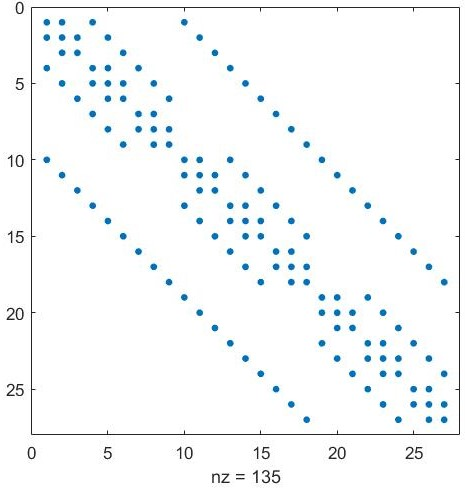
\includegraphics[width=\textwidth]{figures/sparse_8.jpg}
  \end{minipage} %
  \begin{minipage}[b]{0.49\textwidth}
    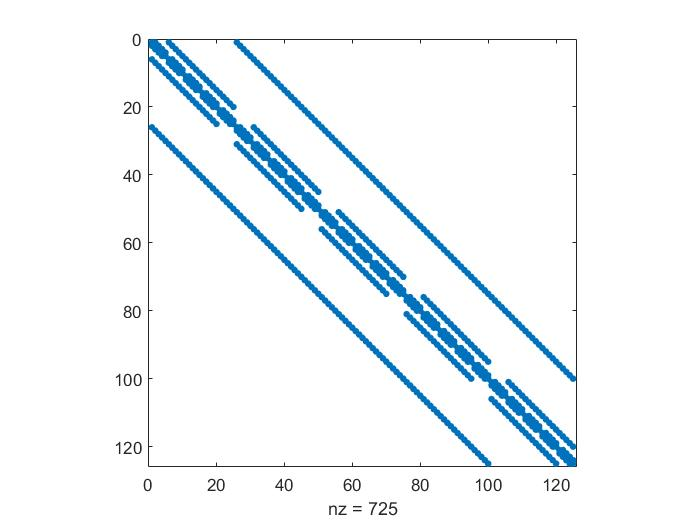
\includegraphics[width=\textwidth]{figures/sparse_64.jpg}

  \end{minipage}
  \caption[Sparse Stencil Matrix]{SINATRA Stencil Matrices, shown through the MATLAB\textsuperscript{\textregistered} spy command (left) 8 Cells in the mesh (right) 64 cells in the mesh.}
  \label{fig:sparse}
\end{figure}


\indent At this stage, the simulation assumes equal cell sizes and refinement across the whole domain. However, the charge density summation is calculated cell by cell, and the electric field is distributed cell by cell. These allow future iterations to have unequal cell sizes. \par


\subsection{Gauss-Seidel}
\label{sec:gauss}

The Gauss-Seidel iterative method was chosen to be the linear algebra solver for SINATRA. It was chosen for it's simplicity, universality, and robustness. It only has one improvement over the simplest iterative method, Jacobi. It solves a version of the equation \(A\cdot x = b\). This thesis will not go into a derivation of the Gauss-Seidel method, but the equation to update the electric potential at each timestep is given by Equation \ref{eqn:gauss_seidel} \footnote{A derivation of the Gauss-Seidel method can be found in Reference \cite{Gauss_eqn}}.

\begin{equation}
    \label{eqn:gauss_seidel}
    x_i^{k+1} = \Big( b_i - \sum_{j=1}^{i-1} A_{i j} x_j^{k+1} - \sum_{j=i+1}^n A_{i j} x_j^{k} \Big) / a_{ii}
\end{equation}

In terms of SINATRA, \\
\(x\) = Electric Potential \\
\(b\) = Charge Density + Boltzman Relationship \\
\(A\) = Stencil \par


\indent The Charge Density (\(b\)) as defined in Equation \ref{eqn:density} involves the electron density, which is assumed to be a fluid currently. It was discussed previously how to distribute the ion's charge, but not how to combine the ion charge and the electron charge. Therefore, by combining Equations \ref{eqn:poisson}, \ref{eqn:density}, and \ref{eqn:e_density} and then discretizing the left hand side of Poisson's Equation, \ref{eqn:poisson} and putting in matrix form, \ref{eqn:stencil}, we get Equation \ref{eqn:mixed}.

\Needspace{5\baselineskip}
\begin{equation}
    \label{eqn:mixed}
    A \cdot \phi = - \frac{e}{\epsilon_0} [n_i - n_o \exp\Big(\frac{\phi - \phi_0}{k \: T_e}\Big)]
\end{equation}
\(A\) = The sparse stencil \\
\(e\) = Charge on an electron \\
\(\epsilon_0\) = Permittivity of free space \\
\(n\) = Number density \\
\(\phi\) = Electric Potential \\
\(\phi_0\) = Initial Electric Potential \\
\(k\) = Boltzmann Constant \\
\(T_e\) = Temperature of the Electrons \par

% capital right hand side?
\indent This shows that the \(b\) in Equation \ref{eqn:gauss_seidel} is the right hand side of the set of linear equations for the Gauss-Seidel solver. Importantly, note that both sides depends on the electric potential. \par
